% GRSL version: hard limit 5 printed pages in the final two-column single-space
% format, INCLUDING references. Do not tweak the style to fit (GRSL editors
% check this explicitly). Cut list vs main.tex: geometric-refinement table,
% adaptive figure, global table + figure, all four appendices, and the
% metric-motivation qualitative figure. Those results survive as prose only.
% Fig. 1 is a figure*[!t] and lands at the top of page 2. IEEE journal style has
% no slot above the abstract (\maketitle owns the top of page 1), and full-width
% floats defer to the next page. A page-1 hero is possible via cuted's `strip`
% (as in main.tex) at the same page count, but deviates from stock GRSL layout.
\documentclass[journal]{IEEEtran}

\usepackage{graphicx}
\usepackage{booktabs}
\usepackage{amsmath}
\usepackage{amssymb}
\usepackage{xcolor}
\usepackage{cite}
\definecolor{tgperi}{HTML}{5A7AB8}
\usepackage[colorlinks=true,citecolor=tgperi,linkcolor=tgperi,urlcolor=tgperi]{hyperref}

\graphicspath{{figures/}}

\begin{document}

\title{FieldVote: Consensus Polygonization for\\ Field Boundary Delineation}

\author{Aviskar~Giri and Isaac~Corley%
\thanks{The authors are with Taylor Geospatial, St.\ Louis, MO 63108 USA
(e-mail: aviskar.giri@taylorgeospatial.org).}}

\markboth{IEEE Geoscience and Remote Sensing Letters}%
{Giri and Corley: FieldVote: Consensus Polygonization for Field Boundary Delineation}

\maketitle

\begin{abstract}
Field-boundary models predict per-pixel probabilities, but downstream users need
polygons, and the conversion between the two largely determines the accuracy of
the delivered product. We study that conversion for a frozen UNet with an
EfficientNet-B7 encoder, retraining nothing. Marker-controlled watershed, the
standard conversion, depends sharply on its h-minima depth, and we find that no
single depth works across regions. FieldVote runs the watershed at $K=14$ depths
and takes a per-pixel majority vote, keeping only boundaries that recur across
the sweep. On the held-out test splits of the ten dense-label Fields of The World
countries it reaches a macro Panoptic Quality of 35.8 against 29.0 for a
per-country tuned watershed, a gain that is significant across countries
(Wilcoxon $p = 0.049$). It needs no labels, no tuning, and no retraining. The
vote also yields a label-free per-field confidence score. We report negative
results: building-derived geometric refinement does not transfer to organic field
boundaries.
\end{abstract}

\begin{IEEEkeywords}
Field boundary delineation, instance segmentation, panoptic quality,
postprocessing, watershed transform.
\end{IEEEkeywords}


\begin{figure*}[!t]
\centering
\centering
\setlength{\tabcolsep}{1.5pt}
\newcommand{\pcell}[1]{\includegraphics[height=1.5in]{#1}}
\begin{tabular}{@{}cccccc@{}}
\pcell{fig_pipe_input.png} & \pcell{fig_pipe_prob.png} &
\pcell{fig_pipe_wslow.png} & \pcell{fig_pipe_wshigh.png} &
\pcell{fig_pipe_consensus.png} & \pcell{fig_pipe_agreement.png} \\[1pt]
\footnotesize Input tile & \footnotesize Field/boundary prob. &
\footnotesize Watershed, low $h$ & \footnotesize Watershed, high $h$ &
\footnotesize FieldVote, $n=11$ & \footnotesize Agreement \\
\end{tabular}
\caption{FieldVote on a held-out Belgium tile. A frozen network maps the input to
a field and boundary probability map; we change only what follows. The watershed
runs at $K$ h-minima depths, of which two are shown: a shallow depth cuts 44
fragments out of the parcels and a deep one merges neighbors. A per-pixel majority
vote keeps only boundaries recurring across the sweep, giving 11 consensus
polygons. The same vote yields a label-free per-field agreement score (green high,
red low) that flags uncertain fields.}
\label{fig:pipeline}
\end{figure*}


\section{Introduction}
\IEEEPARstart{F}{ield} boundaries are the unit of analysis for crop monitoring,
yield estimation, and subsidy administration. Mapping them at scale requires
automated delineation from satellite imagery, and the dominant approach trains a
convolutional network to predict, per pixel, the probability of field interior and
of field boundary~\cite{kerner2024ftw,waldner2020decode}. These probability maps
are well studied, but a cadastre or a yield model consumes vector polygons rather
than rasters of class scores. The step that converts probabilities into polygons
therefore determines the quality of the delivered product, and it has received
far less attention than the network.

That conversion is classically done by marker-controlled watershed seeded at
suppressed minima~\cite{soille2004morphological,koyuncu2016iterative,waldner2020decode}.
Its result depends sharply on the h-minima suppression depth $h$. A shallow depth
over-fragments large fields and a deep one merges small ones, and no single value
is correct across countries: depths suited to the large rectangular fields of
northern Europe over-fragment smallholder regions, and depths suited to
smallholder regions merge large fields into blobs. Tuning $h$ per region would
require ground-truth polygons in every new area, which do not exist at scale,
while a single global depth suits no region in particular. What a practitioner
needs is one label-free rule, with fixed hyperparameters, that works across
regions.

We propose FieldVote. Rather than selecting a depth, we run the watershed at every
depth in a fixed sweep and take a per-pixel majority vote over the resulting
segmentations, keeping only the field boundaries that recur (Fig.~\ref{fig:pipeline}).
Splits that appear at a single shallow depth are voted down; divisions that
persist across the range are retained. The rule adds no learned parameters and
needs no labels. We hold the network frozen and change only the polygonization,
which isolates the contribution of this step.

Our contributions are threefold. First, FieldVote reaches macro Panoptic Quality
(PQ) 35.8 on the held-out test splits of the ten dense-label Fields of The World
countries, against 29.0 for a per-country tuned watershed, a significant gain
obtained without labels or retraining. Second, the same vote agreement provides a
label-free per-field confidence that predicts per-field accuracy within a region.
Third, we report negative results so others need not repeat them: geometric
refinement developed for buildings does not transfer to organic field boundaries,
and simplification compresses geometry sixteen-fold without improving accuracy.


\section{Method}
\label{sec:method}
We postprocess a frozen UNet with an EfficientNet-B7 encoder that emits a
per-pixel softmax over field interior, boundary, and background. The weights stay
fixed and we replace only the conversion of these probabilities into polygons.

\subsection{Threshold-Consensus Polygonization}
Marker-controlled watershed seeds from regional minima after an h-minima
transform, which suppresses minima shallower than a depth
$h$~\cite{koyuncu2016iterative,waldner2020decode}. A single $h$ fixes one point on
the over-segmentation versus under-segmentation trade-off for an entire region.
We instead run the watershed independently at each depth in a fixed set
$H = \{h_1,\dots,h_K\}$, obtaining a label map $L_k$ per run, which we reduce to a
per-pixel field indicator. Writing the vote fraction as
\begin{equation}
\bar{f}(p) = \frac{1}{K}\sum_{k=1}^{K}\mathbb{1}\!\left[p \in \text{field in } L_k\right],
\label{eq:vote}
\end{equation}
the consensus assigns pixel $p$ to field when $\bar{f}(p) \geq \tau_v$, with the
majority vote $\tau_v = 0.5$, and we polygonize the connected components of the
resulting mask. We use the $K = 14$ depths
$H = \{0.5, 0.75, 1, 1.25, 1.5, 2, 4, 8, 12, 16, 24, 32, 48, 64\}$, spanning the
range over which the per-country optimum falls, spaced finely at the shallow end
where the segmentation changes fastest. A sweep of $\tau_v$ from 0.3 to 0.7 leaves
macro PQ flat across the majority region, declining only once more than 60\% of
depths must agree, so 0.5 is a stable operating point rather than a tuned one.
The per-country tuned watershed is the degenerate case $K = 1$. The consensus
recovers the cross-threshold agreement that a single operating point discards, and
adds no learned parameters. It is the spatial analogue of non-maximum
suppression~\cite{neubeck2006nms,solovyev2021wbf}, retaining only detections whose
agreement exceeds a threshold, applied across an operating parameter of one frozen
model rather than across models as in deep
ensembles~\cite{lakshminarayanan2017deepensembles}.

Sweeping a segmentation parameter and combining the results is not itself new.
Hierarchical segmentation builds a nested family of partitions and encodes it as
an ultrametric contour map, from which a single level is then
cut~\cite{arbelaez2011hierarchical,maninis2018cob}, and Koyuncu \emph{et
al.}~\cite{koyuncu2016iterative} sweep the h-minima depth explicitly to expose
over- and under-segmentation as one tunable axis. Those methods use the family to
\emph{choose} an operating point. We keep the family and never choose: the vote
retains the boundaries stable across it, which is why it exceeds even a per-patch
oracle depth (Table~\ref{tab:aggregation}).

\subsection{Threshold-Agreement Confidence}
The sweep also supplies a label-free confidence score. For a consensus field $F$,
its agreement is the fraction of the $K$ runs containing a basin that overlaps $F$
with intersection over union (IoU) at least $\theta = 0.5$,
\begin{equation}
a(F) = \frac{1}{K}\sum_{k=1}^{K}\mathbb{1}\!\left[\exists\, c \in L_k : \mathrm{IoU}(c, F) \geq \theta\right].
\label{eq:agree}
\end{equation}
A field delineated identically at every depth scores $a(F) = 1$. Because $a(F)$
needs no ground truth, it is available wherever the model runs.

\section{Experimental Setup}
\label{sec:setup}
We postprocess one frozen UNet with an EfficientNet-B7 encoder, the PlanetScope
model of Corley \emph{et al.}~\cite{corley_ftp} trained on Fields of The
World~\cite{kerner2024ftw}, operating only on its stored softmax so that every
comparison isolates the polygonization step. The headline comparison uses the
held-out test splits of the ten dense-label countries (\textsc{Dense-10}). We
exclude Kenya, the only presence-only region, whose unlabeled background makes
supervised polygon metrics unreliable~\cite{kerner2024ftw}. Baselines are the
trained-model PlanetScope headline~\cite{corley_ftp}, a per-country tuned
watershed (the best single depth selected per country using ground truth), and
DelineateAnything~\cite{lavreniuk2025delineateanything} on the same imagery in its
default and strongest configurations.

Pixel metrics such as IoU reward correct labeling of large interiors and are
nearly insensitive to whether two adjacent fields are separated. Since the object
of interest is the field, we lead with Panoptic
Quality~\cite{kirillov2019panoptic}, which factors as segmentation quality times
recognition quality (PQ $=$ SQ $\times$ RQ) and penalizes merged and fragmented
fields alike, complemented by average precision (AP) and Boundary
IoU~\cite{cheng2021boundaryiou}. This object-first protocol follows Fields of the
Planet~\cite{corley_ftp} and recent smallholder and pan-European
benchmarks~\cite{persello2023ai4smallfarms,dandrimont2023ai4boundaries}. Macro
scores average per-country values.

\section{Results}
\label{sec:results}

\subsection{FieldVote Improves on a Tuned Watershed}
Table~\ref{tab:main} reports \textsc{Dense-10} results. FieldVote reaches macro PQ
35.8 against 29.0 for the per-country tuned watershed, a gain of 6.8 points that
is significant across countries (Wilcoxon signed-rank $p = 0.049$; bootstrap 95\%
confidence interval on the mean gain $[1.2, 12.1]$). The tuned watershed is the
stronger baseline of the two in the sense that it consumes ground truth to select
its depth, whereas FieldVote uses none. The gain is not confined to PQ: FieldVote
also leads on SQ, RQ, AP, and Boundary IoU, with the largest margin on RQ (44.6
versus 36.6), consistent with the vote correcting instance-count errors rather
than boundary placement. DelineateAnything trails both by a wide margin; it is
trained for a different field regime and transfers poorly to this imagery, so we
report it for context rather than as a competitive baseline.

FieldVote is also within 0.4 points of the trained PlanetScope
model~\cite{corley_ftp}, which scores 35.4 on this backbone and 35.5 on its
EfficientNet-B3 counterpart. We read this as comparable rather than better, since
0.4 points is well inside the spread between those two backbones. The point is
that postprocessing a frozen model recovers trained-model polygon quality at no
training cost.

\begin{table}[t]
\centering
\caption{Polygon-Level Results on \textsc{Dense-10}}
\label{tab:main}
\begin{tabular}{@{}lrrrrr@{}}
\toprule
Method & PQ & SQ & RQ & AP & B-IoU \\
\midrule
DelineateAnything, default~\cite{lavreniuk2025delineateanything} & 5.0 & -- & -- & -- & -- \\
DelineateAnything, strongest~\cite{lavreniuk2025delineateanything} & 14.6 & -- & -- & -- & -- \\
Tuned watershed & 29.0 & 77.0 & 36.6 & 23.2 & 15.6 \\
Trained PlanetScope model~\cite{corley_ftp} & 35.4 & -- & -- & -- & -- \\
\midrule
\textbf{FieldVote (ours)} & \textbf{35.8} & \textbf{77.7} & \textbf{44.6} &
\textbf{29.2} & \textbf{15.9} \\
\bottomrule
\end{tabular}

\smallskip
\begin{minipage}{\columnwidth}
\footnotesize Scores are 0--100; higher is better. The tuned watershed uses
ground truth to select one h-minima depth per country; FieldVote uses no labels.
Macro PQ is the mean of per-country PQ, so it is not exactly SQ $\times$ RQ of
these row averages.
\end{minipage}
\end{table}

\subsection{The Vote, Not the Sweep, Carries the Gain}
Running the watershed at many depths and aggregating the result are separable
choices, so we compare four ways of reducing the same $K = 14$ segmentations to
one (Table~\ref{tab:aggregation}). Pooling the per-depth polygons and suppressing
overlaps by agreement-weighted NMS, and selecting a depth per patch from the elbow
of the instance-count curve, both consume the identical sweep and fall well short
of the vote. The sweep alone is therefore not what produces the gain; how it is
reduced is what matters. The strongest comparison is the per-patch oracle, which
selects the best depth for every patch using ground truth. It is not deployable
and it upper-bounds any method that commits to one depth at a time, yet the
per-pixel vote exceeds it. No choice of operating point, even a clairvoyant one,
recovers what keeping the boundaries that the sweep agrees on recovers.

\begin{table}[t]
\centering
\caption{Aggregation Strategies Over the Same 14-Depth Sweep, \textsc{Dense-10}}
\label{tab:aggregation}
\begin{tabular}{@{}llr@{}}
\toprule
Strategy & Labels used & PQ \\
\midrule
Polygon pool $+$ agreement NMS & none & 24.8 \\
Per-patch elbow selection & none & 26.0 \\
Per-patch oracle depth & ground truth & 30.5 \\
\midrule
\textbf{Per-pixel vote (ours)} & none & \textbf{35.8} \\
\bottomrule
\end{tabular}

\smallskip
\begin{minipage}{\columnwidth}
\footnotesize Scores are 0--100. All four rows reduce the identical set of $K=14$
watershed segmentations; they differ only in how. The oracle selects the
best-scoring depth per patch against ground truth and is reported as an upper
bound on single-depth selection, not as a deployable method.
\end{minipage}
\end{table}

\subsection{Where the Gain Comes From}
Fig.~\ref{fig:percountry} breaks the result down by country. FieldVote wins on 7
of 10, and the aggregate gain comes from suppressing spurious splits in
mid-to-large field regimes rather than from uniform improvement. It gains most
where a single depth over-fragments, in Belgium (30.6 to 52.9) and Croatia (20.5
to 35.8), and loses on the two smallest-field smallholder cases, Cambodia (17.1 to
9.5) and Portugal (12.9 to 9.7), and marginally on Germany (32.5 to 31.2).
Fig.~\ref{fig:results} shows the effect qualitatively: a single depth breaks each
scene into dozens of fragments, splitting the Lithuania tile into 91 pieces, while
the vote recovers 17 parcels that track the annotation.

The headline does not depend on how the ground truth is represented. Scored
against the released per-patch vector polygons instead of connected components of
the rasterized semantic mask, FieldVote reaches 35.5 against 28.6, and the gain
persists on a stricter instance-mask footing (30.0 against 24.4), where both
methods lose absolute points to resampled label edges.

\begin{figure}[t]
\centering
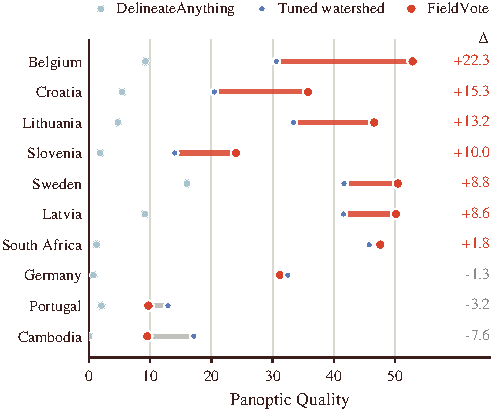
\includegraphics[width=\columnwidth]{fig_percountry.pdf}
\caption{Per-country PQ on \textsc{Dense-10}. FieldVote gains wherever a single
watershed depth over-fragments, most in the mid-to-large field regimes of Belgium
and Croatia, and loses only on the smallest-field smallholder cases (Cambodia,
Portugal) and marginally on Germany.}
\label{fig:percountry}
\end{figure}

\begin{figure}[t]
\centering
\setlength{\tabcolsep}{1pt}
\newcommand{\rcell}[1]{\includegraphics[width=0.325\columnwidth]{#1}}
\begin{tabular}{@{}c@{\,}ccc@{}}
 & \footnotesize Single $h$ & \footnotesize FieldVote & \footnotesize Ground truth \\
\rotatebox{90}{\footnotesize\enspace Belgium} &
\rcell{fig_res_be_single.png} & \rcell{fig_res_be_fv.png} & \rcell{fig_res_be_gt.png} \\
\rotatebox{90}{\footnotesize\enspace Lithuania} &
\rcell{fig_res_lt_single.png} & \rcell{fig_res_lt_fv.png} & \rcell{fig_res_lt_gt.png} \\
\end{tabular}
\caption{Two held-out tiles. A single watershed depth cuts thin spurious splits
across the parcels, breaking the Lithuania scene into 91 pieces; the per-pixel
vote keeps only the boundaries that recur across the sweep and recovers 17
parcels, without retraining or labels.}
\label{fig:results}
\end{figure}

\subsection{Agreement Predicts Per-Field Quality}
Within a country, higher-agreement fields are more accurate. The per-field
Spearman correlation between $a(F)$ and IoU against ground truth is positive and
significant in 5 of the 6 countries tested, from 0.20 (Cambodia) to 0.42
(Slovenia), all $p < 0.0001$; only the smallest test set is not significant
(Rwanda, 174 fields). Across countries the signal does not rank regions by
accuracy, as mean agreement and macro PQ are uncorrelated ($r = 0.07$). Threshold
agreement is therefore a within-region quality estimate, and because it needs no
labels it flags unreliable fields at inference time wherever the model runs.

\subsection{Negative Results}
We tested four refinement operators on the polygon output over 23 countries and
none improved on the raw FieldVote polygons. Douglas--Peucker simplification,
building-style rectilinear regularization~\cite{zorzi2020regularization}, and
Chaikin corner smoothing each moved mean PQ by at most 0.2, and regularization
helped only 1 of 23 countries. The per-country regularization change showed no
significant association with field rectangularity (Pearson $r = 0.135$,
$p = 0.55$, $n = 22$). Building regularizers and frame-field
polygonizers~\cite{girard2021framefield,zorzi2022polyworld} encode a rectilinear
prior that is correct for buildings and wrong for parcels shaped by terrain,
hydrology, and incremental division. Thresholding the boundary-class softmax with
a swept cut instead of taking the argmax changed mean PQ by less than 0.1 across 9
countries, as the consensus over depths already captures that information.
Simplification is worth keeping for compression rather than accuracy: at a 6~m
tolerance it cuts mean vertices per polygon from 188 to 12, a sixteen-fold
reduction, while PQ falls only 0.5.

\subsection{Cross-Sensor Transfer at Global Scale}
FieldVote runs unchanged on the global Fields of The World Sentinel-2 prediction
store~\cite{ftw_global}, a 10~m mosaic of the same three-class softmax produced by
a Sentinel-2 model, which also tests transfer across sensors since we developed the
rule on a PlanetScope model. Table~\ref{tab:global} reports one window per region
across eight agricultural regions on five continents, and the label-free agreement
signal governs the effect. Where agreement is high (95 to 99) the vote
de-fragments, most sharply in Argentina, from 426 to 172 polygons. Where agreement
is low (16 to 42) the predictions are themselves unstable across depths and the
vote produces more and smaller polygons. Agreement therefore indicates where to
apply the rule in deployment. We report polygon counts rather than accuracy here
because global reference parcels are not available.

\begin{table}[t]
\centering
\caption{FieldVote on the Global Sentinel-2 Prediction Store}
\label{tab:global}
\begin{tabular}{@{}lrrrr@{}}
\toprule
Region & Agr. & Tuned WS & FieldVote & Change \\
\midrule
Brazil (Mato Grosso) & 99 & 240 & 208 & $-32$ \\
Argentina (Pampas) & 98 & 426 & 172 & $-254$ \\
Australia (NSW) & 97 & 359 & 319 & $-40$ \\
France & 95 & 416 & 290 & $-126$ \\
\midrule
USA (Iowa) & 87 & 434 & 498 & $+64$ \\
China (Heilongjiang) & 42 & 164 & 355 & $+191$ \\
India (Punjab) & 29 & 20 & 152 & $+132$ \\
Ethiopia & 16 & 31 & 81 & $+50$ \\
\bottomrule
\end{tabular}

\smallskip
\begin{minipage}{\columnwidth}
\footnotesize One 1536$\times$1536 window per region, ordered by agreement.
Columns are polygon counts. Agreement is the label-free score of
(\ref{eq:agree}), in percent. The sign of the count change follows agreement, so
agreement indicates where to apply the vote.
\end{minipage}
\end{table}

\section{Discussion and Limitations}
The best h-minima depth is not a global constant; it shifts with field size,
parcel geometry, and boundary contrast. Committing to one depth commits to one
point on a sharp trade-off, and the wrong point costs PQ. FieldVote sidesteps the
choice by keeping what the sweep agrees on, which filters splits that appear only
at shallow depths and merges that appear only at deep ones. The cost is $K$
watershed runs on a stored softmax, which is inference-time only and embarrassingly
parallel.

FieldVote is not uniformly better. It loses on the smallest-field smallholder
cases, where fields approach the resolution limit and averaging over depths blurs
boundaries that are already
fragile~\cite{persello2023ai4smallfarms,dandrimont2023ai4boundaries}; the gain is
a property of medium-to-large parcel landscapes. A size-adaptive variant recovers
part of that loss by blending the vote with the field probability on patches whose
mean consensus instance area falls below a threshold, a switch that needs no
labels: on a softmax-derived pipeline it raises macro PQ from 33.4 to 35.2, though
on a footing not directly comparable to Table~\ref{tab:main}. We also postprocess
a single frozen model, so we cannot separate errors that postprocessing can fix
from errors already present in the probability map, and PQ can mask systematic
boundary displacement that contour metrics would expose. Finally, the global
evidence of Table~\ref{tab:global} is geometric rather than metric, since
reference parcels are unavailable at that scale; quantifying accuracy there
against independent reference data is future work.

\section{Conclusion}
We treated field-boundary delineation as a polygonization problem on a frozen
model and showed that the conversion from probabilities to polygons, rather than
the network, holds recoverable accuracy. FieldVote, a per-pixel majority vote over
watershed segmentations run at many h-minima depths, raises held-out macro PQ from
29.0 to 35.8 with no labels, no tuning, and no retraining, and supplies a
label-free per-field confidence score as a by-product. Building-derived geometric
refinement does not transfer to organic fields. Extending the consensus to protect
small parcels while retaining the variance reduction that benefits large fields is
the main direction for future work.

\bibliographystyle{IEEEtran}
\bibliography{references}

\end{document}
